\documentclass{projetofinal-dcc}
%%%%%%%%%%%%%%%%%%%%%%%%%%%%%%%%%%%%%%%%%%%%%%%%%%%%%%%%%%%%
%P A C O T E S
%%%%%%%%%%%%%%%%%%%%%%%%%%%%%%%%%%%%%%%%%%%%%%%%%%%%%%%%%%%%
% Adicione aqui seus pacotes

\usepackage{minted}
\usepackage[export]{adjustbox}
\usepackage{float}
%%%%%%%%%%%%%%%%%%%%%%%%%%%%%%%%%%%%%%%%%%%%%%%%%%%%%%%%%%%%
%I N I C I O  D O  D O C U M E N T O
%%%%%%%%%%%%%%%%%%%%%%%%%%%%%%%%%%%%%%%%%%%%%%%%%%%%%%%%%%%%
\begin{document}

% título da tese é obrigatório
\title{Título}

% autor é obrigatório; máximo de 3 autores
\author{Filipe Xavier Trindade dos Santos }{[Aqui entram os agradecimentos]}
\author{Lucas Simões de Sousa Arnaud }{[Aqui entram os agradecimentos]}
\author{Thales Teixeira Pires}{[Aqui entram os agradecimentos]}

% orientador é obrigatório
\advisor[Profª.]{Silvana Rosseto,~Ph.D.}{}

% co-orientador é opcional
%\coadvisor[Prof.]{Nome do co-orientador,~M.Sc.}{}

% máximo de 3 integrantes da banca (orientador e co-orientador já são adicionados automaticamente)
\banca[Prof.]{Nome do participante banca 1,~D.Sc.}{COPPE~-~UFRJ}
\banca[Prof.]{Nome do participante banca 2,~Ph.D.}{COPPE~-~UFRJ}
%\banca[Prof.]{Nome do participante banca 3,~Ph.D.}{COPPE~-~UFRJ}

\location{Rio~de~Janeiro}{RJ}{Brasil}

% mês e ano de defesa
\date{junho}{2016}
\maketitle

\startdocument
%%%%%%%%%%%%%%%%%%%%%%%%%%%%%%%%%%%%%%%%%%%%%%%%%%%%%%%%%%%%
%A G R A D E C I M E N T O S
%%%%%%%%%%%%%%%%%%%%%%%%%%%%%%%%%%%%%%%%%%%%%%%%%%%%%%%%%%%% 
\makethankspage

%%%%%%%%%%%%%%%%%%%%%%%%%%%%%%%%%%%%%%%%%%%%%%%%%%%%%%%%%%%%
%R E S U M O
%%%%%%%%%%%%%%%%%%%%%%%%%%%%%%%%%%%%%%%%%%%%%%%%%%%%%%%%%%%%
\begin{abstract}{
  A eficiência de uma empresa está diretamente relacionada à forma como são conduzidos os seus processos internos. Quanto maior o tamanho da organização, mais importante se torna a sua capacidade de gestão para garantir que eles sejam executados com correção e dentro dos prazos esperados. Uma abordagem efetiva para atingir a eficiência organizacional é a automatização de processos de negócio.

O objetivo deste trabalho é apresentar duas diferentes tecnologias já existentes utilizadas para automatização de processos, o Redmine e os chamados BPMS, e suas principais características, e propor uma forma de integração entre elas, aproveitando as qualidades de ambas para oferecer maior qualidade de gestão, padronização e otimização de recursos na execução de processos de negócio.
}
\end{abstract}

%%%%%%%%%%%%%%%%%%%%%%%%%%%%%%%%%%%%%%%%%%%%%%%%%%%%%%%%%%%%
%A B S T R A C T
%%%%%%%%%%%%%%%%%%%%%%%%%%%%%%%%%%%%%%%%%%%%%%%%%%%%%%%%%%%%
\begin{englishabstract}{
  The efficiency of a company is directly related to the way its internal processes are conducted. The larger the size of the organization, the more important its management capacity becomes to ensure that they are executed with correctness and within the expected time frames. An effective approach to achieving organizational efficiency is the automation of business processes.

The objective of this work is to present two different technologies used for automation of processes, Redmine and the so-called BPMS, and their main characteristics, and to propose a way of integration between them, taking advantage of the qualities of both to offer higher management quality, standardization and optimization of resources in the execution of business processes.
}
\end{englishabstract}

%%%%%%%%%%%%%%%%%%%%%%%%%%%%%%%%%%%%%%%%%%%%%%%%%%%%%%%%%%%%
%L I S T A S
%%%%%%%%%%%%%%%%%%%%%%%%%%%%%%%%%%%%%%%%%%%%%%%%%%%%%%%%%%%%
% Figuras
\makefigurespage

% Tabelas
\maketablespage

% Algoritmos
\makelistingspage

% Abreviaturas (devem estar em ordem alfabética)
\makeabrevpage{\item [BPM] Business Process Management
\item [BPMS] Business Process Management System
\item [BPMI] Business Process Management Initiative
\item [BPMN] Business Process Management Notation
\item [XML] Extensible Markup Language
\item [OMG] Object Management Group


}

% Símbolos (devem estar em ordem alfabética)
% \makesymbolspage{\input{elementos-pretextuais/simbolos}}

% Sumário 
\maketocpage

%%%%%%%%%%%%%%%%%%%%%%%%%%%%%%%%%%%%%%%%%%%%%%%%%%%%%%%%%%%%
%C O N T E Ú D O
%%%%%%%%%%%%%%%%%%%%%%%%%%%%%%%%%%%%%%%%%%%%%%%%%%%%%%%%%%%%
\startcontent
\chapter{Introdução}\label{chp:introducao}

\section{Motivação}\label{sec:introducao-motivacao}
Os processos de negócio consistem numa sequência de atividades e serviços que  encadeados cumprem determinado objetivo ou função na organização em que é desempenhado. A automatização de processos de negócio consiste na aplicação de tecnologia, de forma que uma ou mais atividades de um processo possam ser automatizadas, reduzindo assim a dependência de atuação humana para sua execução.

\section{Objetivos}\label{sec:introducao-objetivo}
O objetivo geral deste trabalho é propor uma solução para automatização de processos complexos que também contam com interação humana, inclusive durante o fluxo destes. Vamos apresentar uma ferramenta que permite a modelagem de fluxos variados, facilita a configuração e implementação, bem como a utilização contínua por usuários com conhecimentos básicos de processo e o acompanhamento deste por um gerente.

\section{Organização do texto}\label{sec:introducao-organizacao_texto}
\chapter{Automatização de processos}\label{chp:conceitos_basicos}


\section{Processos}\label{sec:conceitos_basicos-processos}
Processo de negócio é um conjunto de atividades coordenadas, relacionadas entre si, que envolvem diferentes pessoas, procedimentos, áreas e tecnologias com o objetivo de gerar valor para a empresa, seja em forma de produtos ou serviços, internos ou externos.

\section{BPM}\label{sec:conceitos_basicos-bpm}
BPM é o acrônimo para o inglês Business Process Management, ou gestão de processos de negócio em português. Seu principal objetivo é oferecer uma abordagem sistemática para a execução, adaptação e melhoria de processos de negócio em um ambiente de constantes mudanças. O BPM pode ser encarado sob duas perspectivas distintas: o BPM como engenharia de software ou o BPM como disciplina de gestão.

\section{BPMn}\label{sec:automatizacao-processos-bpmn}

\section{BPMS}\label{sec:automatizacao-processos-bpms}
\subsection{Activiti BPM}\label{sec:automatizacao-processos-bpms-activiti}

O Activiti BPM é uma ferramenta BPMS open-source, utilizada na automatização de processos de negócio em um sistema de informação. Tem por objetivo prover um motor BPM leve, estável e fácil de integrar em diferentes tipos de aplicações e ambientes. A versão 5.19 foi utilizada neste trabalho.



\section{Redmine}\label{sec:conceitos_basicos-redmine}
O Redmine\cite{redmine} é uma ferramenta de gerenciamento de projetos open-source. Foi criada por Jean-Philippe Lang em 2006. Desenvolvido em Ruby, utilizando a framework Rails, tem como objetivo dar flexibilidade de configuração ao usuário, e também ao desenvolvedor. A versão 3.1 deste software foi utilizada neste trabalho.



\chapter{Problema}\label{chp:problema}

\section{Introdução}\label{sec:problema-introducao}

As organizações, sejam de grandes dimensões ou não, são constituídas por recursos humanos e não-humanos que interagem entre si, através do compartilhamento de recursos físicos ou virtuais, como por exemplo na troca de informações operacionais entre diferentes áreas de uma empresa. Cada uma dessas interações definem processos de negócio que tem por objetivo produzir um resultado para os envolvidos nessa interação extra ou intra-organizacional.

Os processos de negócio, quando realizados de forma desorganizada e despadronizada, levam à ineficiência organizacional pelo simples fato de sua execução não otimizada. Isso ocasiona em elevação dos custos, aumento no retrabalho, insatisfação dos colaboradores e a consequente diminuição na qualidade dos serviços relacionados. Portanto, torna-se altamente necessário uma boa gestão dos processos, a fim de que esses problemas sejam evitados ou mitigados a tempo e não tornem-se um câncer corporativo.

O acesso mais rápido e eficiente às informações estabelece melhores condições para a execução de processos de negócio. Entretanto, não é suficiente para evitar problemas inerentes à presença de informação. A execução despadronizada de processos sem o apoio de um sistema de informação, ou mesmo suportada por sistemas de informação que não acompanham a flexibilidade da constante mudança dos processos, são em geral gargalos fundamentais no insucesso das diversas organizações existentes. A solução desses problemas estabelece melhores condições para a execução, monitoramento e controle de processos, o que termina por aperfeiçoar a tomada de decisão no nível estratégico organizacional.

Neste trabalho, apresentaremos uma alternativa para garantir que a execução das atividades das empresas sejam realizadas da maneira esperada e aumentar a capacidade de monitoramento de cada uma das etapas, que é a automatização de processos. 

\section{Caso de Uso}\label{sec:problema-caso_de_uso}

Ao longo deste trabalho, iremos utilizar o processo descrito a seguir como caso de uso para cada uma das demonstrações de automatização das ferramentas utilizadas para o desenvolvimento da solução proposta.

Em um cenário de operação de um portal de e-commerce, é muito importante a gestão dos preços praticados pela empresa nas diferentes categorias que compõe o mix de produtos ofertados ao consumidor. Erros cometidos por uma precificação manual indevida podem levar a altos prejuízos financeiros e ações na justiça por parte dos consumidores, além de afetar a imagem da corporação perante o mercado. 

O caso ocorrido com a gigante Walmart no portal brasileiro em dezembro de 2013, exemplifica bem o cenário descrito no parágrafo anterior. Neste caso, um computador que custava R\$2.398 reais foi anunciado por R\$580, o que representava um diferença de 75\% a menor em relação ao valor original. Este caso foi noticiado pela imprensa na época, e também houve bastante repercusão nas redes sociais, deixando muitos clientes insatisfeitos pelo cancelamento da compra (http://oglobo.globo.com/economia/defesa-do-consumidor/walmart-erra-preco-de-produto-em-site-cancela-venda-irrita-clientes-11098550). 

Nesse sentido, torna-se necessária a implantação de um processo de precificação manual que envolva a avaliação de regras que limitem a troca de preço sem a aprovação de alçadas superiores. Essa nova gestão tem por objetivo trazer mais qualidade e segurança nas mudanças de preço solicitadas pelos diferentes precificadores das categorias do site, alinhando assim a gestão de preços do portal e evitando trocas de preço equivocadas ou não autorizadas pelos gestores.

O processo inicia com a decisão do analista de uma determinada categoria de produtos do site, pela mudança de preço de um SKU. O novo preço do SKU é definido pelo analista e enviado para aprovação.

A solicitação enviada pelo analista é avaliada quanto a regra de alçada definida pelos gestores, e caso possua uma variação de preço acima de 30\%, deve passar pela aprovação de dois gestores. Em um cenário real de negócios, certamente a regra seria mais complexa, como por exemplo variando em função da categoria do produto. Entretanto, assumiremos a regra da variação de 30\% nas demonstrações como forma de simplificar o entendimento e aplicação das regras de negócio estabelecidas para o processo.

Após a avaliação da variação de preço, caso tenha sido acima de 30\%, o processo deve ser encaminhado para a aprovação de dois gestores. Caso a variação seja menor ou igual a 30\%, a mudança não requer aprovação. Após isso, a troca de preço será efetuada no portal.

A imagem a seguir descreve de forma visual o fluxo do processo descrito anteriormente:

\begin{figure}[H]
  \centering
  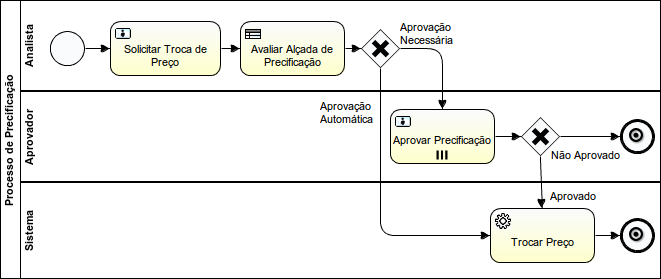
\includegraphics[width=1.0\textwidth]{imagens/ProcessoDePrecificacao.png}
  \caption{Processo de Precificação Manual}
  \label{fig:exemplo_bpmn}
\end{figure}
\chapter{Redmine}\label{chp:redmine}

\section{Introdução}\label{sec:redmine-introducao}
Neste capítulo vamos explicar como o Redmine, uma ferramenta de gerenciamento de projetos foi utilizada para gestão de processos, ilustrando com um exemplo. Vamos apresentar ainda, a capacidade extensiva desta ferramenta através do desenvolvimento de plugins. Por último vamos abordar as limitações do Redmine que nos motivaram a desenvolver algo novo para atingir nosso objetivo em automatização de processos.

\section{Estrutura básica do Redmine}\label{sec:redmine-estrutura_basica}

A estrutura básica de gerenciamento de projetos no Redmine é composta por X principais elementos. São eles:

\subsection{Tarefas}\label{subsection:redmine-estrutura_basica-tarefa}

São as unidades básicas de execução de trabalho dos projetos (\ref{subsection:redmine-estrutura_basica-projeto}). Elas contém os dados relevantes para o seu gerenciamento (e.g, tipo (\ref{subsection:redmine-estrutura_basica-tracker}, situação(\ref{subsection:redmine-estrutura_basica-status}), data de início, data de conclusão, categoria), para a sua execução (e.g, título, descrição) e dados adicionais que podem variar entre os projetos e tipos de tarefa, que são cadastrados como campos personalizados (\ref{subsection:redmine-estrutura_basica-custom_fields}).  

\subsection{Projetos}\label{subsection:redmine-estrutura_basica-projeto}

\subsection{Tipos de tarefa}\label{subsection:redmine-estrutura_basica-tracker}

\subsection{Situação}\label{subsection:redmine-estrutura_basica-status}

\subsection{Papéis de usuários}\label{subsection:redmine-estrutura_basica-role}

\subsection{Campos Customizados}\label{subsection:redmine-estrutura_basica-custom_fields}


\section{Gestão de processos com o Redmine}\label{sec:redmine-gestao_processos}


\section{Como automatizar um processo?}\label{sec:redmine-automatizar_processo}

\section{Plugins}\label{sec:redmine-plugins}
O Redmine foi desenvolvido de forma a ser extensível por meio de plugins. É possível modificar um funcionalidade da ferramenta, ou criar novas funcionalidades sem precisar alterar o código desta. Os plugins são desenvolvidos em Rails, a mesma linguagem de programação do Redmine. 

Para possibilitar extensões de funcionalidades que envolvem enxertar pedaços de código no meio de uma classe ou de uma tela, o Redmine disponibiliza hooks em diversas partes da ferramenta. São tags com um identificador da parte do código em que estão inseridas. E para utilizar este hook basta incluir um hook listener num plugin, e direcionar qual arquivo ou método um determinado hook vai disparar.

\section{Limitações}\label{sec:redmine-limitacoes}


\chapter{Activiti BPM}\label{chp:activiti}

\section{Introdução}\label{sec:activiti-introducao}
Criado em 2010 por ex-integrantes do projeto jBPM, o Activiti BPM é um projeto de código aberto sob a licença Apache V2, que provê um motor BPM leve e completo sob a especificação BPMN 2.0. O Activiti é desenvolvido sob a linguagem de programação Java e é facilmente integrável com aplicações existentes por sua leveza e API amigável.

Neste capítulo vamos apresentar como o Activiti BPM pode ser utilizado na automatização de processos de negócio. Vamos apresentar ainda, a capacidade de modelagem de processos através da notação BPMN utilizada pelo Activiti. Por último vamos abordar as vantagens e limitações desta ferramenta frente às demais opções do mercado.

\section{BPMN}\label{sec:activiti-bpmn}
A BPMN (Business Process Management Notation) foi criada para representar processos de negócio em forma de diagrama, através de uma notação padronizada e de fácil entendimento por diferentes profissionais, sejam desenvolvedores, analistas de negócio ou gestores. Foi criada inicialmente pelo BPMI (Business Process Management Initiative) em 2004, mas atualmente é mantida e atualizada pela OMG (Object Management Group). Sua versão mais atual é a BPMN 2.0, publicada em 2011.

A notação foi concebida sob a perspectiva de cobrir a falta de entendimento entre diferentes departamentos e organizações a cerca de um determinado processo ou conjunto de processos, algo muito frequente no ambiente corporativo. Além disso, através de sua notação padronizada em XML (Extensible Markup Language), diferentes ferramentas podem fazer o uso de sua auto-descrição para orquestração de processos de negócio, sejam eles automatizáveis ou não.

A notação define quatro grupos distintos de objetos para permitir a diagramação de um fluxo de negócio. Os objetos são classificados em artefatos, agrupadores, conectores e objetos de fluxo. São utilizadas figuras geométricas, como retângulos e círculos, além de linhas pontilhadas e tracejadas, entre outros elementos para representar cada um dos objetos que constituem a notação.

1) http://searchcio.techtarget.com/definition/Business-Process-Modeling-Notation

2) http://blog.iprocess.com.br/2012/11/um-guia-para-iniciar-estudos-em-bpmn-i-atividades-e-sequencia

3) https://www.fluig.com/blog/entendendo-melhor-o-bpmn/

\begin{figure}
  \centering
  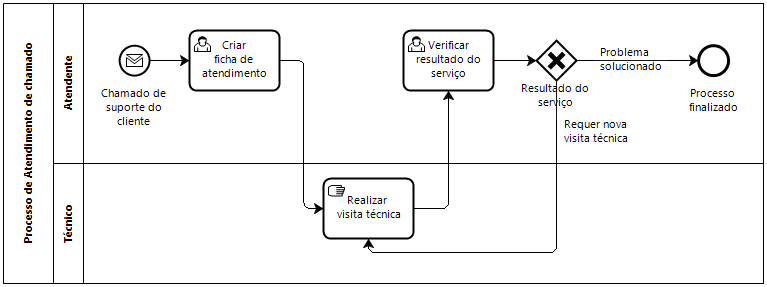
\includegraphics[width=1.0\textwidth]{imagens/bpmn_example.png}
  \caption{Exemplo de processo representado em BPMN}
  \label{fig:exemplo_bpmn}
\end{figure}

\section{Gestão de processos com o Activiti BPM}\label{sec:activiti-gestao_processos}

O motor do Activiti BPM é disponibilizado através de um simples arquivo JAR, modelo de arquivo padrão para bibliotecas da linguaguem Java. Sendo assim, o motor BPM pode ser facilmente utilizado em diferentes projetos Java através da inclusão dessa biblioteca como dependência e pela utilização de sua API.
\section{Como automatizar um processo?}\label{sec:activiti-automatizar_processo}

\section{Vantagens e Limitações}\label{sec:activiti-vantages_limitacoes}



\chapter{Integração Redmine e Activiti BPM}\label{chp:integracao_redmine_activiti}

\section{Introdução}\label{sec:integracao_redmine_activiti-introducao}
Dadas as vantagens e limitações das ferramentas Activiti e Redmine utilizadas como plataformas para a automatização de processos, decidimos desenvolver uma forma de integrá-las para explorarmos os pontos positivos de cada uma delas.

Para atingir este objetivo, criamos um plugin para o Redmine que possibilita a comunicação com o Activiti. Nas próximas sessões, descreveremos o processo de construção deste plugin e como utilizá-lo.


\section{Customização do Redmine}\label{sec:integracao_redmine_activiti-implementacao}

A integração tem por objetivo centralizar o máximo de funcionalidades no Redmine, deixando transparente tanto para o usuário comum como o gestor, a existência de um motor BPM por trás.

\subsection{Funcionalidades}\label{sec:integracao_redmine_activiti_implementacao_funcionalidades}
\subsubsection{Conexão com o Activiti }\label{sec:integracao_redmine_activiti_inplementacao_funcionalidades_conexão}
Para iniciar a utilização do plugin é necessário configurar os detalhes para conexão com o Activiti BPM.
Após colocar o servidor, login e senha, também é preciso disparar os jobs que rodam continuamente para sincronizar os processos e tarefas entre o Redmine e o Activiti.

\subsubsection{Configuração dos estados}\label{sec:integracao_redmine_activiti_inplementacao_funcionalidades_conexão}
Também é necessário configurar os estados principais a serem utilizados pelo plugin.
Configure os estados padrão que devem ser utilizados quando um processo é criado, concluído ou está em andamento.

\subsubsection{Deploy de um processo}\label{sec:integracao_redmine_activiti_inplementacao_funcionalidades_deploy}
Como já foi explicado, o processo deve ser modelado na notação BPMN. Mas à partir deste ponto, toda a interação será através do Redmine.
Na tela de processos, ao clicar em Novo processo, é possível fazer upload de uma modelagem de um processo para o Redmine. Esta operação tenta o deploy do arquivo selecionado no Activiti, através do serviço REST e apresenta o resultado na tela.

A cada vez que esta tela é atualizada, a lista de processos é atualizada. Nela são mostrados todo os fluxos de trabalho ativos no BPMS, inclusive os que não foram instalados através da interface citada acima. Ao clicar numa linha, o usuário consegue visualizar o diagrama do processo.

É possível efetuar o deploy da mesma definição de processo mais de uma vez, caso sejam feitas alterações no fluxo. Neste caso, o novo deploy será identificado como uma nova versão do mesmo processo. 

\subsubsection{Configuração de um processo}\label{sec:integracao_redmine_activiti_inplementacao_funcionalidades_configuracao}
A integração das duas ferramentas se dá na sincronização dos processos e tarefas humanas do Activiti. A representação para elas que foi implementada no Redmine é explicada nas duas seções a seguir:

\begin{itemize}
\item \textbf{Representação de um processo} - Um fluxo de um processo modelado e instalado no Activiti é chamado de definição de processo. No Redmine, o tipo da tarefa representa a definição de processo, e determinará qual o processo que é disparado na criação de uma tarefa. Uma instância (a materialização de uma definição de processo) de um processo no BPMS é iniciada pela criação de uma tarefa no Redmine. Durante toda a vida de um processo, este é representado pela tarefa que deu início a ele. 

\item \textbf{Representação de uma tarefa humana} - Quando um fluxo vai para uma etapa de tarefa humana, é criado uma tarefa no Redmine para representá-la e aonde a interação necessária com o usuário acontecerá. Esta tarefa será filha da tarefa que representa a instância do processo em questão.
\end{itemize}

A primeira configuração a ser feita consiste em definir qual o tipo de tarefa estará conectado ao processo sendo editado. Além disso, é exibida a lista de versões do processo selecionado, e qual a versão ativa. Ao estabelecer esta conexão, toda tarefa deste tipo criada no Redmine disparará uma instância dessa definição de processo no Activiti, na versão ativa marcada.
Na mesma tela também é possível redefinir o nome que aparece na lista de processos.

O próximo passo é editar uma versão para configurar mais detalhes:

\begin{itemize}
\item \textbf{Ativo} - Como explicado anteriormente, ao marcar esta opção, o usuário estabelece a versão padrão que deve ser disparada pelas tarefas conectadas a este processo.

\item \textbf{Variáveis do processo} - Numa definição de um processo podem ser definidas diferentes variáveis a serem usadas para definir o status ou responsável de uma tarefa, para preencher automaticamente um campo ou tomada de decisão. Devem ser preenchidos os valores para essas variáveis utilizadas no processo de acordo com o tipo definido.

\item \textbf{Estados de conclusão do processo} - 
Na modelagem do processo podem ser configurados diferentes eventos de término. Nesta seção são configurados quais status no Redmine vão representar cada evento.

\item \textbf{Configuração das tarefas do processo} - 
Aqui são listadas as etapas do tipo tarefa humana presentes na modelagem. Para cada uma é possível definir o status com o qual deve ser criada cada sub-tarefa que representa a tarefa humana em questão, e definir um tipo de tarefa diferente para cada uma. Caso o campo \textbf{Tipo} não seja preenchido, a sub-tarefa será do mesmo tipo da tarefa original. Caso contrário, a sub-tarefa terá o tipo definido, que pode ser usado para representar um novo processo.

\item \textbf{Campos personalizados utilizados pelo processo} - Na modelagem, o evento de inicialização, bem como as tarefas humanas de um processo possuem campos de formulário. Os valores destes campos são sincronizados junto com as tarefas do Redmine para o Activiti e vice-versa. Para guardar estes campos nas tarefas do Redmine são utilizados campos personalizados. Nesta seção portanto, deve ser selecionado cada campo customizado que representará os campos definidos no processo.

\end{itemize}

\subsection{Detalhes do desenvolvimento}\label{sec:integracao_redmine_activiti_implementacao_detalhes_desenvolvimento}

\subsubsection{Linguagens}\label{sec:integracao_redmine_activiti_implementacao_detalhes_desenvolvimento_linguagens}

O plugin desenvolvido para Redmine foi desenvolvido em Ruby\cite{ruby-lang}, utilizando a framework Rails\cite{rails}. A linguagem open source e orientada a objetos, disponibilizada ao público em 1995, foi criada por Yukihiro “Matz” Matsumoto, inspirada nas linguagens Perl, Smalltalk, Eiffel, Ada e Lisp, suas linguagens preferidas. Em 2006, o Ruby atingiu aceitação massiva, com a formação de grupos de usuários em todas as principais cidades do mundo e com as conferências sobre Ruby com lotação esgotada. Ruby está entre as 10 linguagens mais populares, segundo o índice TIOBE\cite{tiobe} de abril de 2016, que se baseia nas buscas com o nome da linguagem como palavra chave. A framework Rails é uma biblioteca (ou gema) que extende de Ruby. Foi criada por David Heinemeier Hansson em 2004 para a utilização desta linguagem para o desenvolvimento de aplicações web. Isto é feito através da comunicação da comunicação do Ruby com HTML, CSS e Javascript.

As modificações feitas no Activiti foram feitas em Java, a linguagem que em que este foi desenvolvido. Criado em 1995 por um time da Sun (chamado de "Green Team"), Java\cite{java-history} é uma linguagem interpretada orientada a objetos,  que é independente de plataforma, pois sempre executa na JVM (Java Virtual Machine). Segundo o índice TIOBE de abril de 2016 é a linguagem mais popular no mundo.

\subsubsection{Banco de dados}\label{sec:integracao_redmine_activiti_implementacao_detalhes_desenvolvimento_bd}

\subsubsection{Sincronizacao}\label{sec:integracao_redmine_activiti_implementacao_detalhes_desenvolvimento_sincronizacao}

\paragraph{Definição de processo}

% Ao fazer o deploy de um processo através da interface do Redmine é disparado um serviço que acessa a API REST do Activiti, executando uma requisição POST que efetivamente executa o deploy, adicionando a modelagem do processo em questão à lista de definições de processos ativos, que podem ser iniciados.

% O código a seguir monta a requisição POST repository/deployments enviando o arquivo .bpmn, que retorna o deployment\_id do processo cujo deploy acaba de ser feito.

% \codejava{Ruby}{alg:LABEL_CODE_5}{codigos/deploy_process.rb}


% Após executado o serviço é iniciado um job que acessa, através de um outro serviço que busca a definição à partir do deployment\_id. As informações do processo que são recuperadas consistem das tarefas humanas definidas, campos de formulário, variáveis de processo e outros detalhes.

% O código a seguir monta a requisição GET que recupera a definição de um processo.

% \codejava{Ruby}{alg:LABEL_CODE_4}{codigos/process_definition_by_deployment_id.rb}

% O código a seguir consiste do job que centraliza a sincronização de uma definição de processo no momento do deploy. 

% \codejava{Ruby}{alg:LABEL_CODE_3}{codigos/sinchronize_process_definition_job.rb}


\paragraph{Tarefas humanas}\label{sec:integracao_redmine_activiti_implementacao_detalhes_desenvolvimento_sincronizaca_human_task}

\paragraph{Inicialização de um processo}\label{sec:integracao_redmine_activiti_implementacao_detalhes_desenvolvimento_sincronizacao_processo}
% Sempre que uma tarefa é criada, caso ela esteja vinculada a um processo BPM, um serviço é disparado. Este serviço executa 


\subsubsection{Configuracao do processo}\label{sec:integracao_redmine_activiti_implementacao_detalhes_desenvolvimento_configuracao}
% Escrever sobre os detalhes de como modelar um processo que se comunica com o Redmine

\section{Customização do Activiti}\label{sec:integracao_redmine_activiti-implementacao-activiti}

A integração entre o Redmine e o Activiti BPM foi desenvolvida sob o aspecto de direcionar a maior parte das customizações para o lado do Redmine, uma vez que esta é apenas uma das possibilidades de interface com o motor de processos. Num cenário mais amplo de processos mais complexos, outros tipos de dispositivos ou sistemas poderiam realizar uma comunicação direta com os processos.

A API REST padrão oferecida pelo Activiti foi utilizada para a integração entre as ferramentas, uma vez que é bem completa e oferece a maioria dos serviços necessários para a comunicação. Também contou a facilidade de chamadas a APIs REST pelo Ruby on Rails. 

Entretanto, identificamos a ausência de um serviço fundamental para integração entre as ferramentas. Esse serviço deveria retornar uma lista contendo as definições de tarefas contidas em um determinado processo, incluindo os campos disponíveis nos formulários das tarefas. Essa definição nos permitiria estabelecer a interface para o mapeamento dos campos do processo com os campos das tarefas do Redmine.

Sendo assim, extendemos a API REST do Activiti, através da criação de um classe Java representando um novo serviço, semelhante aos serviços existentes no seu código-fonte. Esse serviço consistiu no consumo de uma API Java já disponibilizada pelo Activiti, mas ausente na API REST. O código-fonte simplificado desta classe pode ser observado abaixo:

\codejava{Java}{alg:LABEL_CODE_2}{codigos/TaskDefinitionService.java}

\section{Resultados}\label{sec:integracao_redmine_activiti-resultados}
\chapter{Lorem ipsum dolor sit amet}\label{chp:LABEL_CHP_2}

\section{Tables}\label{sec:LABEL_CHP_2_SEC_A}
Reference: \url{http://en.wikibooks.org/wiki/LaTeX/Tables}

\begin{table}[!h]
  \centering
  \begin{tabular}{ |l|l|l| }
    \hline
      Goalkeeper & Alan Smith & Paul Robinson \\
    \hline
      Lucus Radebe &  Mark Viduka & Michael Duberry \\
    \hline
      Eirik Bakke & Jamie McMaster & Jody Morris \\
    \hline
  \end{tabular}
  \caption{This table shows some data}
  \label{tab:LABEL_TAB_1}
\end{table}

\section{Images}\label{sec:LABEL_CHP_2_SEC_B}
Reference: \url{http://en.wikibooks.org/wiki/LaTeX/Importing_Graphics}

\begin{figure}
  \centering
%  \includegraphics[width=0.6\textwidth]{imagens/chick.png}
  \caption{Chick}
  \label{fig:LABEL_FIG_1}
\end{figure}

\section{Equations}\label{sec:LABEL_CHP_2_SEC_C}
Reference: \url{http://en.wikibooks.org/wiki/LaTeX/Mathematics}

Also: \url{http://en.wikibooks.org/wiki/LaTeX/Advanced_Mathematics}

\begin{equation}
  (x + y)^2 = x^2 + 2xy + y^2
  \label{eq:LABEL_EQ_1}
\end{equation}

\section{Listings}\label{sec:LABEL_CHP_2_SEC_D}
Reference: \url{http://en.wikibooks.org/wiki/LaTeX/Source_Code_Listings}

\codec{C}{alg:LABEL_CODE_1}{codigos/codigo-c.txt}

\codejava{Java}{alg:LABEL_CODE_2}{codigos/codigo-java.txt}

\section{References}\label{sec:LABEL_CHP_2_SEC_E}
\begin{itemize}
  \item Referencing \refchapter{chp:LABEL_CHP_1}
  \item Referencing \refsection{sec:LABEL_CHP_1_SEC_A}
  \item Referencing \refsection{sec:LABEL_CHP_1_SEC_C}
  \item Referencing \reftable{tab:LABEL_TAB_1}
  \item Referencing \reffigure{fig:LABEL_FIG_1}
  \item Referencing \refequation{eq:LABEL_EQ_1}
  \item Referencing \reflisting{alg:LABEL_CODE_1}
  \item Referencing \refappendix{chp:LABEL_APP_1}
\end{itemize}
\pagebreak

%%%%%%%%%%%%%%%%%%%%%%%%%%%%%%%%%%%%%%%%%%%%%%%%%%%%%%%%%%%%
% B I B L I O G R A F I A
%%%%%%%%%%%%%%%%%%%%%%%%%%%%%%%%%%%%%%%%%%%%%%%%%%%%%%%%%%%%
% Retirar esta parte se o trabalho não tiver bibliografia
%\bibliographystyle{ieeetr}
%\bibliography{referencias}
\makebibspage{abnt}{elementos-postextuais/referencias}

%%%%%%%%%%%%%%%%%%%%%%%%%%%%%%%%%%%%%%%%%%%%%%%%%%%%%%%%%%%%
% A P E N D I C E
%%%%%%%%%%%%%%%%%%%%%%%%%%%%%%%%%%%%%%%%%%%%%%%%%%%%%%%%%%%%
% Retirar esta parte se o trabalho não tiver anexos
\appendix
\chapter{Processo de Precificação em BPMN}\label{chp:LABEL_APP_1}

    \lstset{
    language=xml,
    tabsize=3,
    %frame=lines,
    caption=Código do Processo de Precificação em BPMN,
    label=code:process_bpmn,
    frame=shadowbox,
    rulesepcolor=\color{gray},
    xleftmargin=20pt,
    framexleftmargin=15pt,
    keywordstyle=\color{blue}\bf,
    commentstyle=\color{OliveGreen},
    stringstyle=\color{red},
    numbers=left,
    numberstyle=\tiny,
    numbersep=5pt,
    breaklines=true,
    showstringspaces=false,
    basicstyle=\footnotesize,
    emphstyle={\color{magenta}}}
    \lstinputlisting{codigos/process.xml}

\chapter{REST de Definições de Tarefas}\label{chp:LABEL_APP_1}

     \lstset{
    language=java,
    tabsize=3,
    %frame=lines,
    caption=REST de Definições de Tarefas,
    label=code:task_definition_service,
    frame=shadowbox,
    rulesepcolor=\color{gray},
    xleftmargin=20pt,
    framexleftmargin=15pt,
    keywordstyle=\color{blue}\bf,
    commentstyle=\color{OliveGreen},
    stringstyle=\color{red},
    numbers=left,
    numberstyle=\tiny,
    numbersep=5pt,
    breaklines=true,
    showstringspaces=false,
    basicstyle=\footnotesize,
    emphstyle={\color{magenta}}}
    \lstinputlisting{codigos/TaskDefinitionService.java}

\end{document}